
\fullcite{momy93} \\

Note that Harder is co-author here and author of the previous subsection \label{ve_hard91}
which explains the overlap in notations.

%-------------------
\begin{multicols}{2}
\begin{center}
{\bf Article excerpts}
\\ 
{\bf Notes and remarks}
\end{center}
\end{multicols}

%-------------------
\begin{multicols}{2}
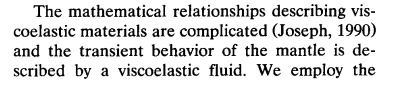
\includegraphics[width=7cm]{images/viscoelasticity/momy93a}\\
\end{multicols}

%-------------------
\begin{multicols}{2}
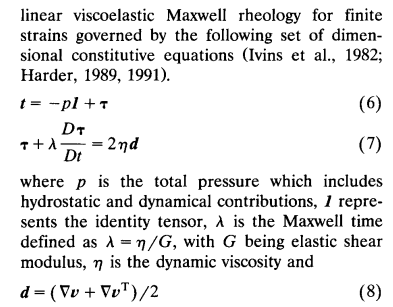
\includegraphics[width=7cm]{images/viscoelasticity/momy93b}\\
\[
{\bm \sigma} = -p {\bm 1} + {\bm \tau}
\]
\[
{\bm \tau}  + \frac{\eta}{\mu} \frac{{\cal D} {\bm \tau}}{{\cal D}t} = 2\eta \dot{\bm \varepsilon}
\Rightarrow
\frac{1}{2\eta} {\bm \tau}  + \frac{1}{2\mu} \frac{{\cal D} {\bm \tau}}{{\cal D}t} 
=  \dot{\bm \varepsilon}
\]
\end{multicols}

%-------------------
\begin{multicols}{2}
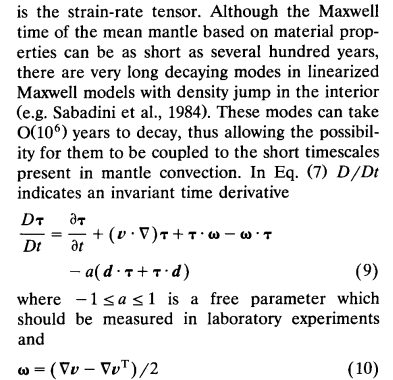
\includegraphics[width=7cm]{images/viscoelasticity/momy93c}\\
\[
\frac{{\cal D} {\bm \tau}}{{\cal D}t} = \frac{\partial {\bm \tau}}{\partial t}  
+ (\vec\upnu \cdot \vec\nabla) {\bm \tau} 
+ {\bm \tau} \cdot \dot{\bm \omega} + \dot{\bm \omega} \cdot {\bm \tau}
- a (\dot{\bm \varepsilon} \cdot {\bm \tau} + {\bm \tau} \cdot \dot{\bm \varepsilon})
\]
\[
\dot{\bm \omega} = \frac12 (\vec\nabla \vec\upnu  - \vec\nabla \vec\upnu^T  ) 
\]
\end{multicols}

